As mentioned in the previous chapter, molecular dynamics simulation is 
a numerical system that describe atomic status over time in a specified 
environment. From the cultivated information, we can either investigate 
the atomic behaviors or calculate thermophysics properties such as thermal 
conductivity and viscosity easily. A standard molecular dynamics simulation 
has an algorithm as follows \cite{manjunatha_development_2018}
\begin{figure}
    \begin{center}
        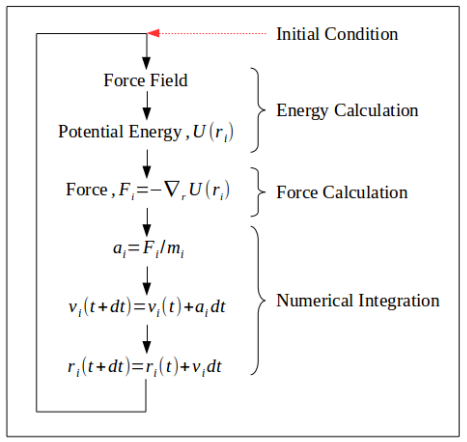
\includegraphics[width=0.75\textwidth]{mdalgo.png}
    \end{center}
    \caption{Basic outline of a MD simulation}
\end{figure}
\newpage
The initial conditions describe the initial state of the atoms such as 
velocity $v(t_0)$, mass of atom $m$ and coordination $r(t_0)$. For atoms of a liquid, given the $i^{th}$ atom, 
the initial coordination $r_i(t_0)$ is randomized along with several 
constraints such as structural constraints (angles, bond lengths) 
and displacement constraints to avoid malfunction in the system as well as 
systematic errors. The initial velocity $v_i(t_0)$ is randomized on the Gaussian 
distribution with the constraint that the total momentum of the entire system 
is $0$.

After the initial setup, a class of functions called a force field is used 
to calculate the potential energy $U_i = U(r_i)$ which is a function of position 
that obeys the structural constraints of the atom. The obtained potential 
energy $U(r_i)$ can be used to deduce the forces $F_i$ that apply on the atom.

The force $F_i$ is then processed by using Verlet algorithm as follows to obtain 
the functions of velocity and position over time. For a time step $\Delta t$, 
the function that presents the position of the $i^{th}$ atom after $\Delta t$ is
\begin{equation}
    r_{i}(t+\Delta t) \approx r_{i}(t)+\Delta t \dot{r}_{i}(t)+\frac{1}{2} \Delta t^{2} \ddot{r}_{i}(t)\label{eq:2.1.1}
\end{equation}
To get the velocity term after a time step $\Delta t$, we have to deduce $r_i(t)$ 
backwards from $r_i(t+\Delta t)$. Thus
\begin{equation}
    r_{i}(t) \approx r_{i}(t+\Delta t)-\Delta t \dot{r}_{i}(t+\Delta t)+\frac{1}{2} \Delta t^{2} \ddot{r}_{i}(t+\Delta t)\label{eq:2.1.2}
\end{equation}
Substituting \ref{eq:2.1.2} into \ref{eq:2.1.1} we get
\begin{equation}
    \dot{r}_{i}(t+\Delta t)=\dot{r}_{i}(t)+\frac{1}{2} \Delta t\left[\ddot{r}_{i}(t)+\ddot{r}_{i}(t+\Delta t)\right]
\end{equation}
Or
\begin{equation}
    \dot{r}_{i}(t+\Delta t)=v_{i}(t+\Delta t)=v_{i}(t)+\frac{1}{2 m_{i}} \Delta t\left[F_{i}(t)+F_{i}(t+\Delta t)\right]
\end{equation}
The values of positions and velocities at $t+\Delta t$ will be served as the next 
initial condition for the next loop of calculation until the set running time 
T is reached. The values of positions and velocities will be used to calculate 
thermal conductivity and viscosity by using a deduction of the Green-Kubo 
relation.